\documentclass[12pt,a4paper]{article}
\usepackage[utf8]{inputenc}
\usepackage[T1]{fontenc}
\usepackage[portuguese]{babel}
\usepackage{graphicx}
\usepackage{grffile} % Adicionado para garantir que o compilador aceite os sublinhados (_) nos nomes das imagens
\usepackage{geometry}
\geometry{a4paper, margin=2.5cm}
\usepackage{hyperref}

\begin{document}

\begin{titlepage}
    \centering
    \vspace*{2cm}
    
    {\Large \textbf{[NOME DA SUA UNIVERSIDADE]}}\\[0.5cm]
    {\large Curso de [Nome do Curso]}\\[3cm]
    
    {\Large \textbf{Integrantes do Grupo:}}\\[0.5cm]
    Vitor Alexandre Moreira Amaral \\
    Pedro Henrique Bellone Souza e Silva \\
    Edson Pimenta Almeida \\
    Nalberth Henrique Vieira Pinto \\
    Yan Sabarense Coelho Silva \\[3cm]
    
    {\huge \textbf{Trabalho Prático I - Roteamento}}\\[1.5cm]
    
    {\large \textbf{Disciplina:} Redes de Computadores I}\\[0.5cm]
    {\large \textbf{Professor:} Max do Val Machado}
    
    \vfill
    
    {\large [Cidade - Estado]}\\[0.5cm]
    {\large Junho de 2026}
\end{titlepage}

\newpage

\section{Objetivo}
O objetivo deste trabalho prático é consolidar os conceitos de infraestrutura de redes e desenvolvimento de aplicações distribuídas. O projeto engloba a configuração de uma topologia de rede utilizando o Cisco Packet Tracer, implementando roteamento estático e redirecionamento de portas (Port Forwarding), bem como o desenvolvimento de uma aplicação cliente-servidor em Java. A aplicação utiliza multithreading e os protocolos da camada de transporte TCP e UDP para demonstrar o envio e recebimento simultâneo de mensagens em uma rede simulada e, posteriormente, analisada via Wireshark.

\section{Metodologia e Topologia (Fase 1)}
A topologia exigida no projeto foi adaptada para utilizar dois roteadores (R1 e R3) e dois computadores (PC1 e PC2), mantendo o particionamento em três redes distintas (192.168.0.0/16, 172.16.0.0/12 e 10.0.0.0/8).

\begin{itemize}
  \item \textbf{Configuração Base:} O PC1 atua como cliente na rede 192.168.0.0/16 (via gateway R1). O PC2 atua como servidor na rede 10.0.0.0/8 (via gateway R3). O R1 e R3 interconectam-se através da rede 172.16.0.0/12.
  \item \textbf{Roteamento Estático:} Foram adicionadas rotas estáticas em R1 e R3 para permitir que pacotes originados no PC1 cheguem ao PC2 e vice-versa.
  \item \textbf{Port Forwarding:} Foi configurado o NAT Estático nos roteadores para redirecionar o tráfego destinado à porta da aplicação para o IP correto dentro da topologia, permitindo a comunicação fim a fim do cliente com o servidor.
\end{itemize}

\begin{figure}[h!]
\centering
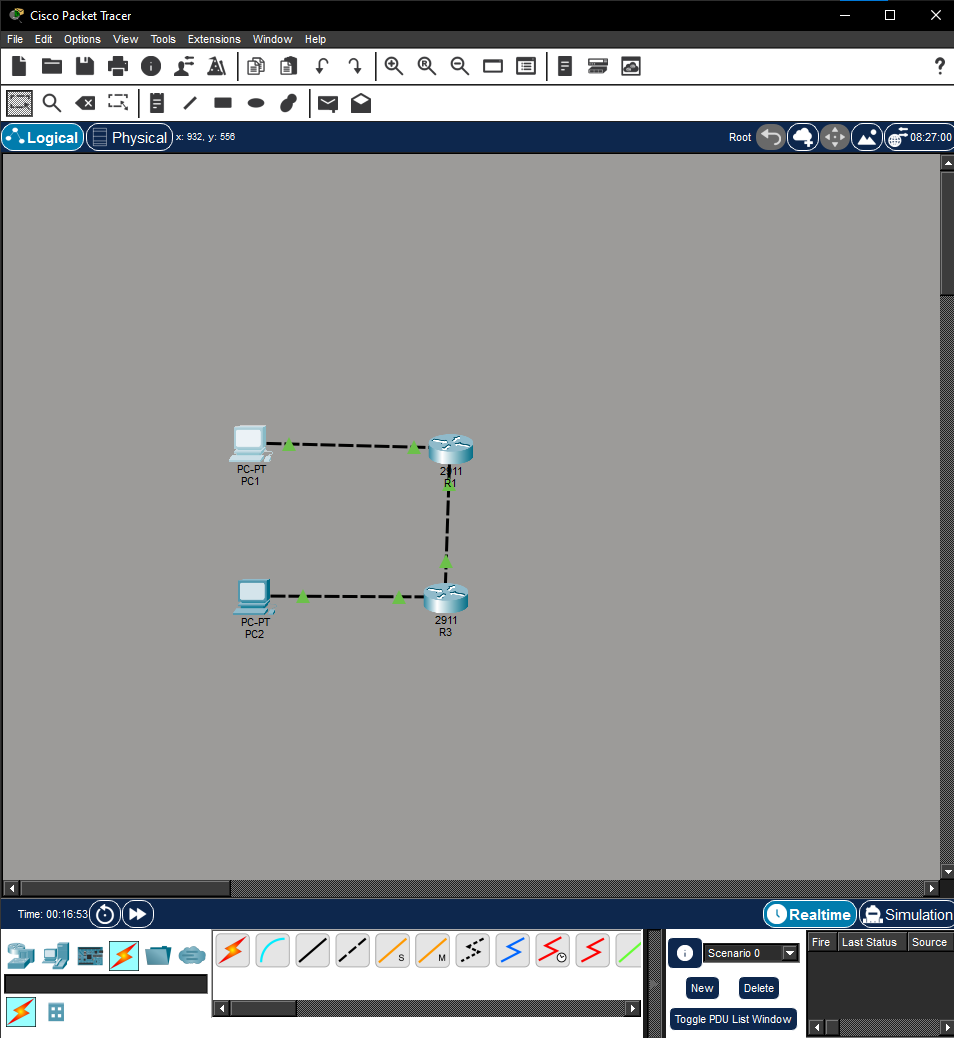
\includegraphics[width=\textwidth]{imgs/projeto_completo_cisco.png}
\caption{Topologia Completa no Cisco Packet Tracer}
\end{figure}

\begin{figure}[h!]
\centering
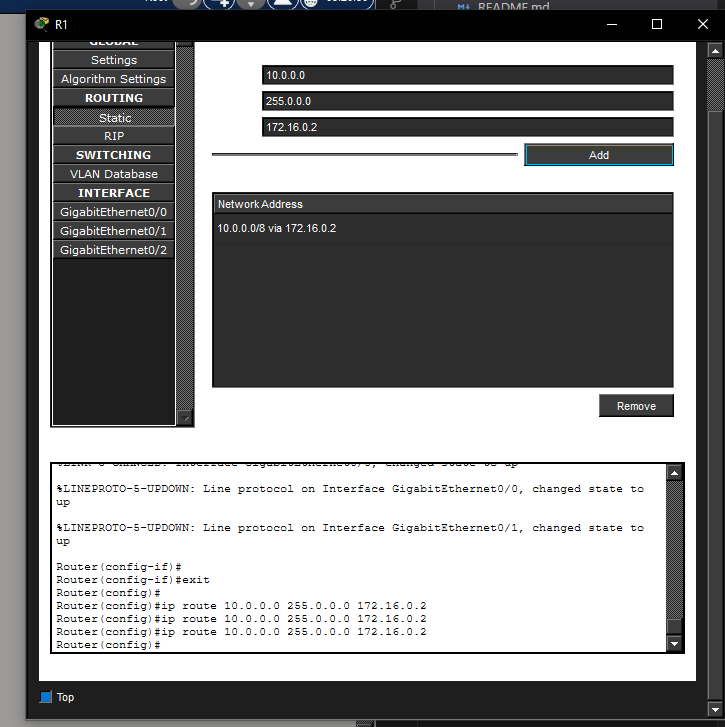
\includegraphics[width=\textwidth]{imgs/routing_static_1.png}
\caption{Configuração de Roteamento Estático - R1}
\end{figure}

\begin{figure}[h!]
\centering
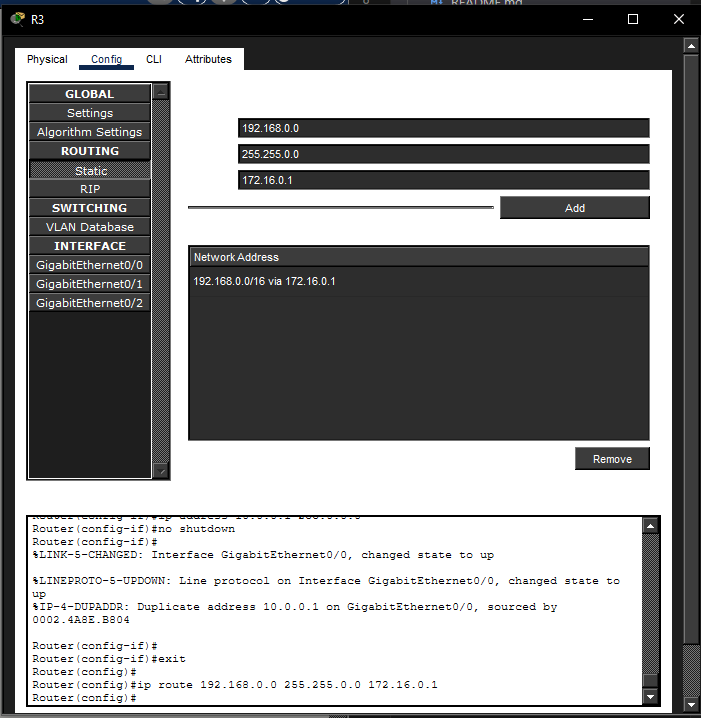
\includegraphics[width=\textwidth]{imgs/routing_static_2.png}
\caption{Configuração de Roteamento Estático - R3}
\end{figure}

\begin{figure}[h!]
\centering
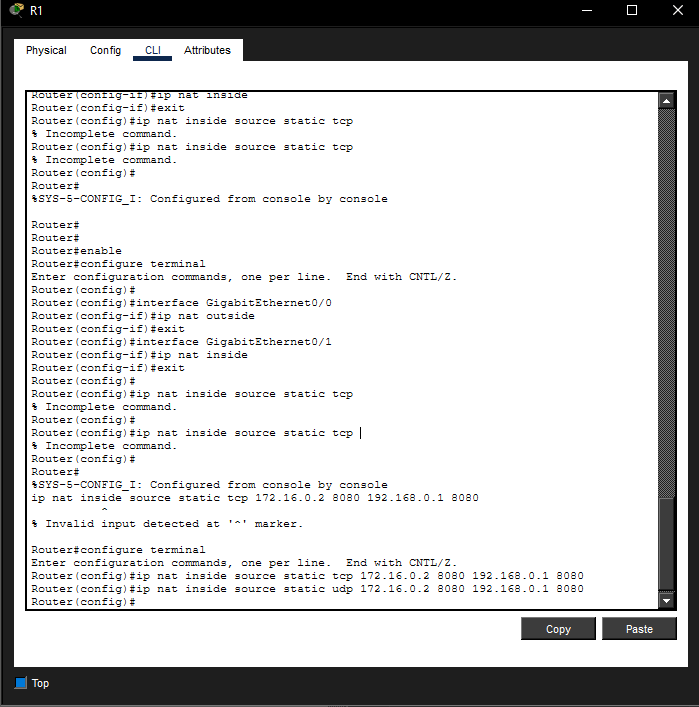
\includegraphics[width=\textwidth]{imgs/CLI_packet_tracer.png}
\caption{Configuração de Port Forwarding (NAT) via CLI}
\end{figure}

\section{Desenvolvimento de Software (Fase 2)}
A aplicação foi construída em Java utilizando a biblioteca Swing para a interface gráfica do cliente (\texttt{Cliente.java}) e Java padrão para o Servidor (\texttt{Servidor.java}).

Para suprir o requisito de escutar e processar requisições TCP e UDP simultaneamente na mesma máquina, o \texttt{Servidor.java} foi desenvolvido utilizando \textbf{Multithreading}. Ao ser iniciado, o programa principal ramifica duas novas \textit{Threads}: a primeira inicializa um \texttt{ServerSocket} ouvindo na porta TCP 5000, e a segunda inicializa um \texttt{DatagramSocket} ouvindo na porta UDP 5001.

No lado do cliente, botões independentes na interface gráfica capturam o IP de destino e a mensagem digitada, instanciando requisições TCP ou UDP em \textit{Threads} separadas, garantindo que a janela do cliente não congele ("freeze") durante a espera pela resposta da rede.

\begin{figure}[h!]
\centering
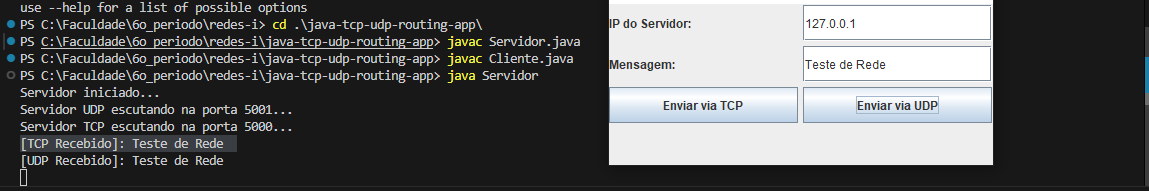
\includegraphics[width=\textwidth]{imgs/cliente_servidor_terminal.png}
\caption{Aplicação Cliente e Servidor em Execução}
\end{figure}

\section{Avaliação de Tráfego (Fase 3)}
Para a validação prática, utilizou-se o software Radmin VPN para emular o roteamento entre dois computadores físicos distintos em redes remotas, criando um túnel seguro para tráfego local (LAN). Com a VPN ativa, o cliente conectou-se ao IP fornecido pela rede virtual ao PC servidor.

O tráfego de rede gerado pela aplicação Java foi inspecionado utilizando o analisador de protocolos \textbf{Wireshark}. A ferramenta foi filtrada para escutar unicamente as portas alvo da aplicação (\texttt{tcp.port == 5000 or udp.port == 5001}).

\begin{figure}[h!]
\centering
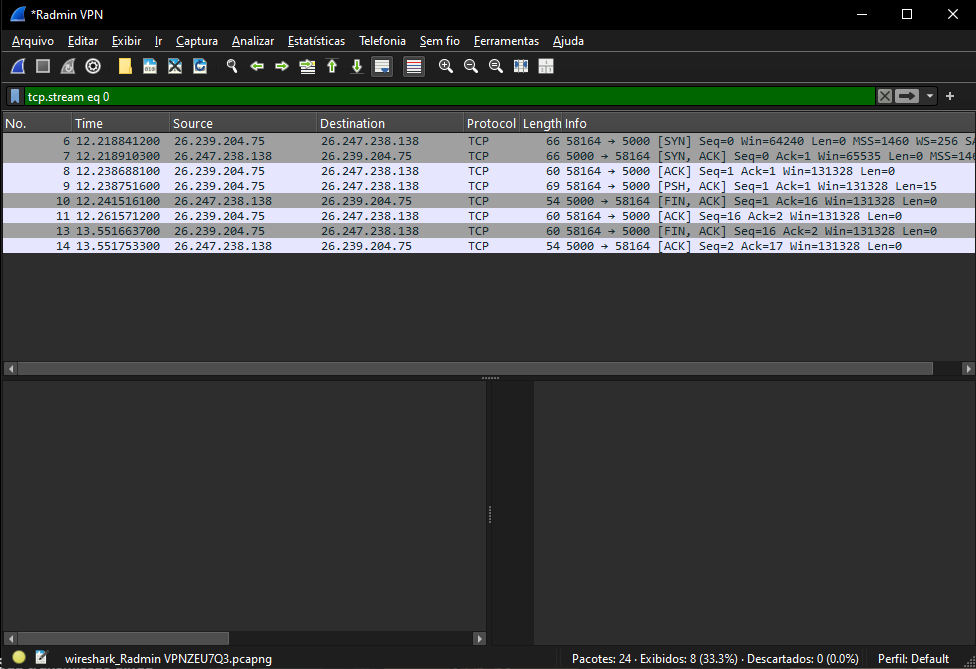
\includegraphics[width=\textwidth]{imgs/wireshark1.png}
\caption{Análise do Wireshark - Captura 1}
\end{figure}

\begin{figure}[h!]
\centering
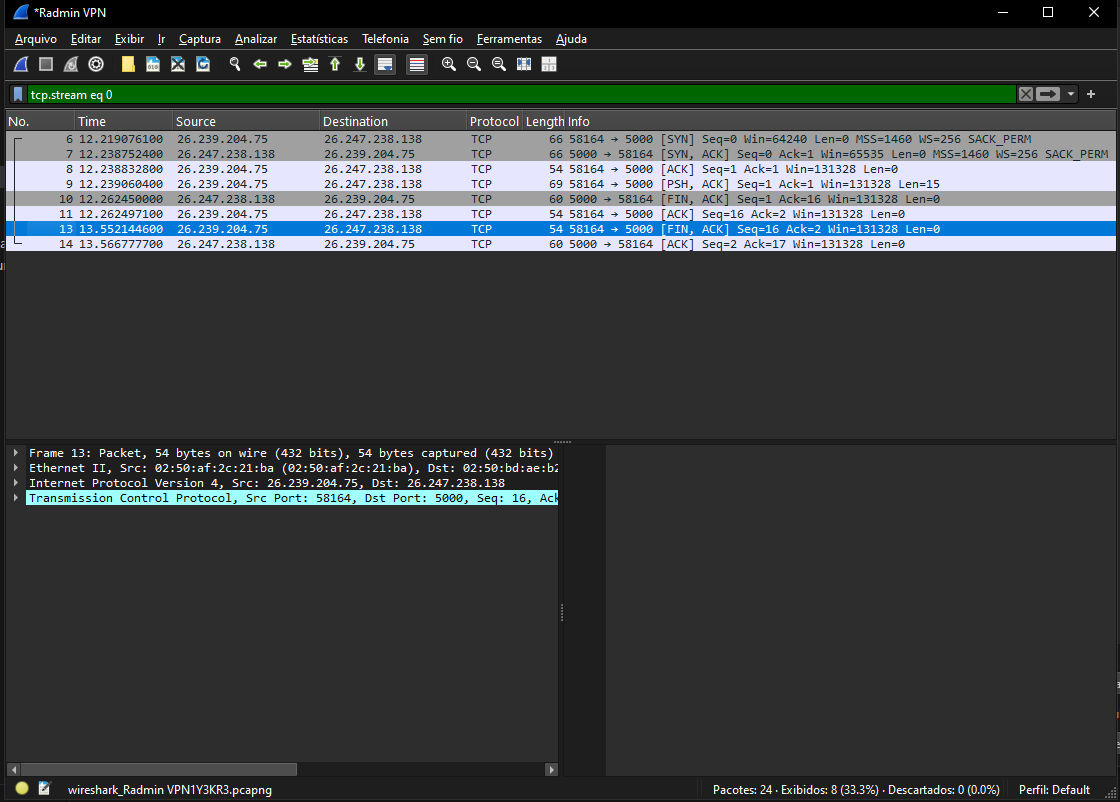
\includegraphics[width=\textwidth]{imgs/wireshark2.png}
\caption{Análise do Wireshark - Captura 2}
\end{figure}

\begin{figure}[h!]
\centering
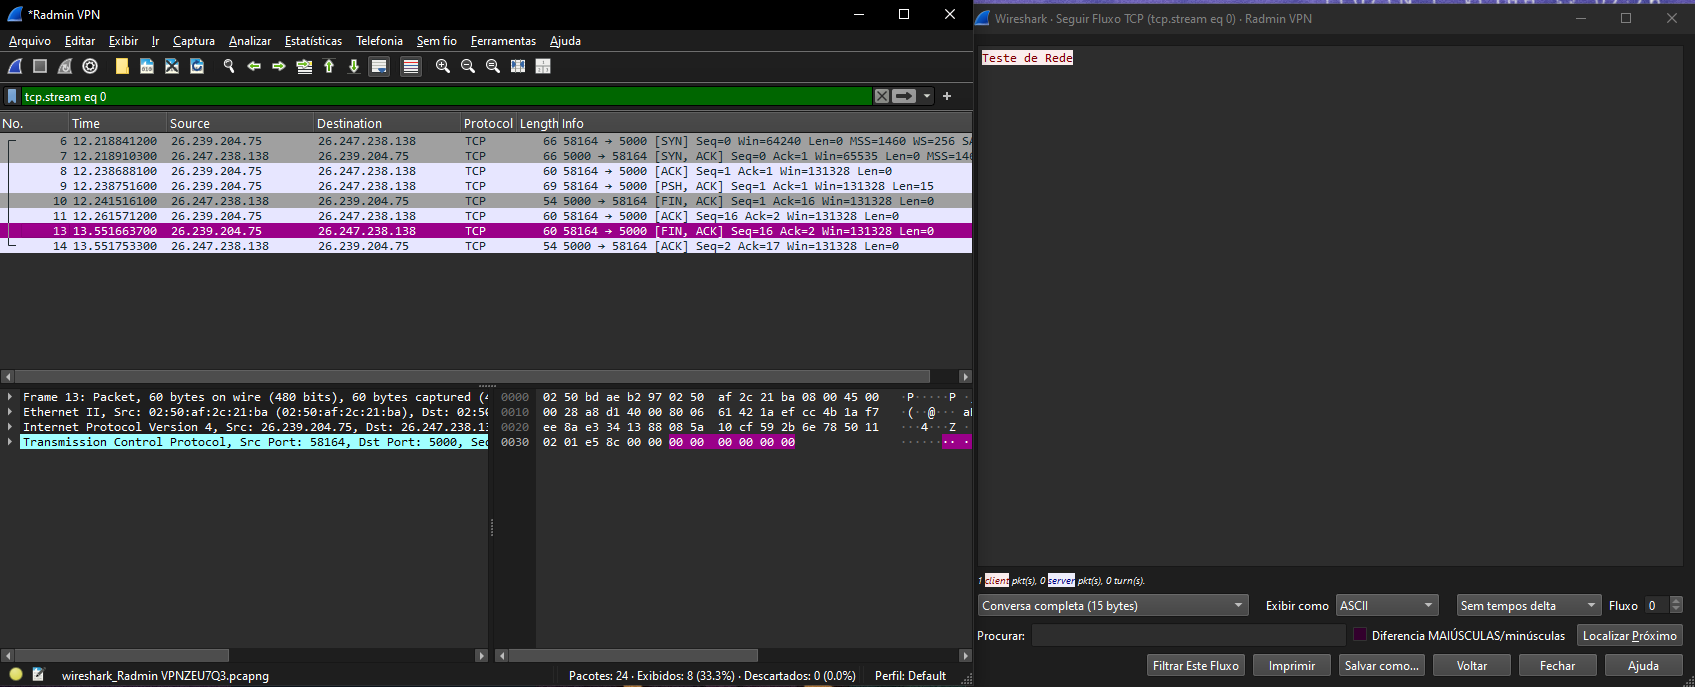
\includegraphics[width=\textwidth]{imgs/wireshark3.png}
\caption{Análise do Wireshark - Captura 3}
\end{figure}

\begin{figure}[h!]
\centering
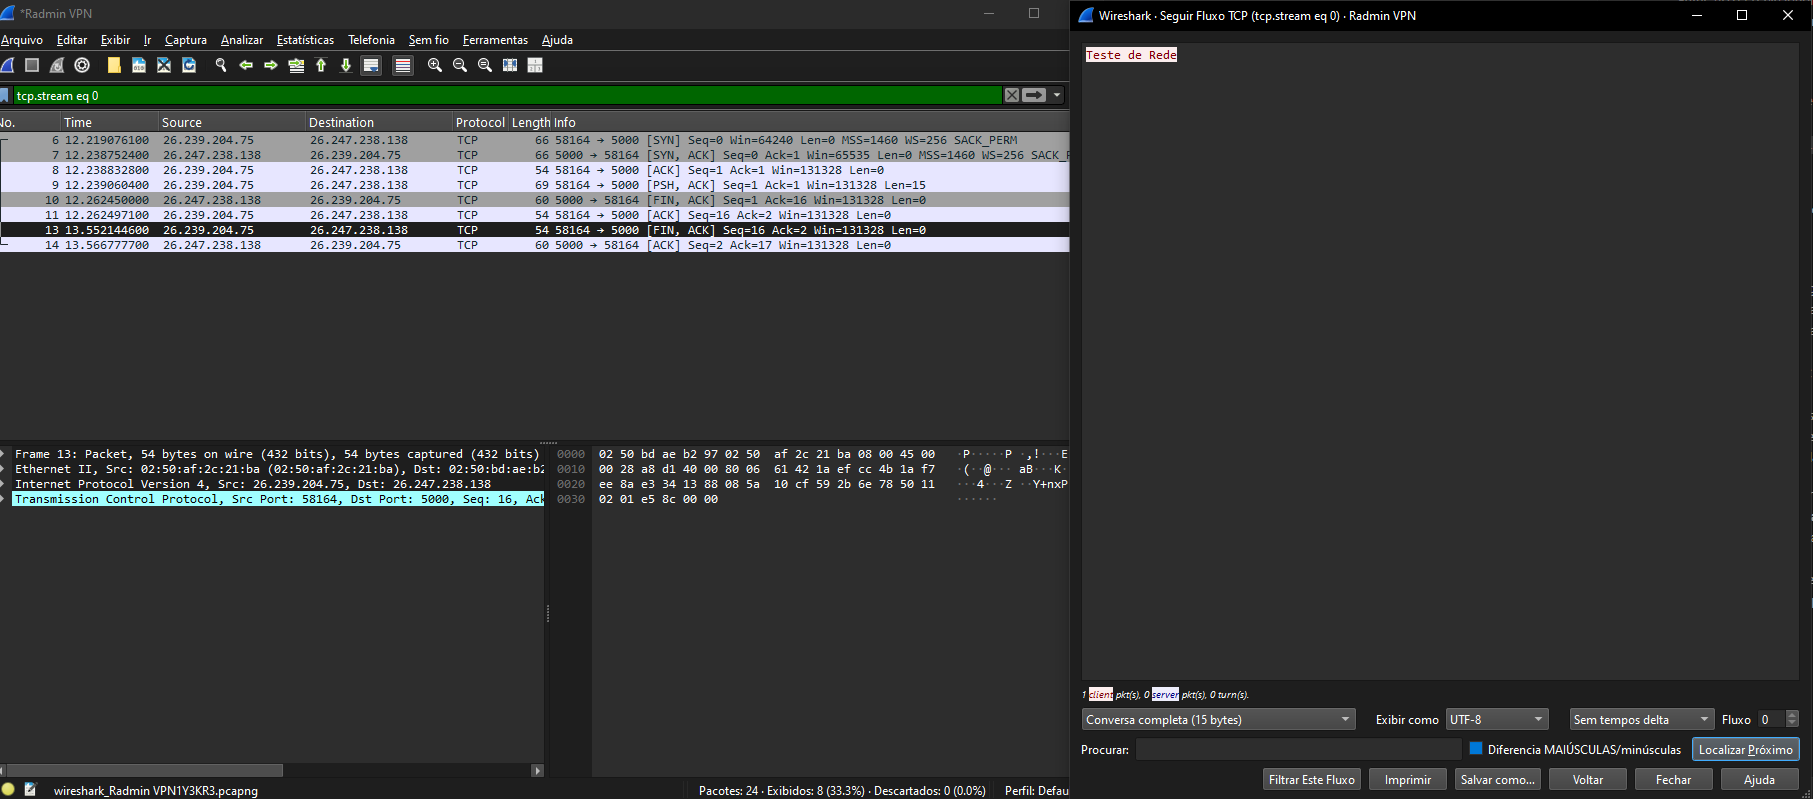
\includegraphics[width=\textwidth]{imgs/wireshark4.png}
\caption{Análise do Wireshark - Captura 4}
\end{figure}

\section{Conclusão}
Durante a realização deste trabalho, foi possível transpor o conhecimento teórico para um ambiente de simulação e prática. Os principais desafios encontrados envolveram:

\begin{enumerate}
  \item A configuração de NAT Estático e compreensão de interfaces \textit{inside} e \textit{outside} no terminal do Cisco Packet Tracer.
  \item O entendimento das configurações de rede da máquina para evitar conflitos de IP na simulação ("Duplicate Address").
  \item A manipulação correta das \textit{Threads} no Java para garantir a escuta paralela dos dois protocolos.
\end{enumerate}

Esses obstáculos foram solucionados através da análise minuciosa dos logs de erro do terminal (como logs do roteador e CLI) e debug da comunicação de rede através de pings segmentados, confirmando que a união de conceitos de roteamento infraestrutural e chamadas de sockets em software funcionam em uníssono para promover a comunicação de dados.

\end{document}
